During the development process of a framework for web-based human and machine
computation the first issue that needed to be
resolved was the description of a suitable model for supporting such framework.
The design of a model involves the definition of the data structures that will
be used by the workflow, and of course the definition of the workflow itself.

\subsection{Data Design}
In the design process for the data model we faced the problem of creating a
suitable underlying model for all the application need that we have to cover,
spacing from pure \acl{HC} task to \emph{parasitic computing}. This wide range
of possible applications and the need of great flexibility demanded to the system,
led us to the creation of a meta model for almost all the data structures used in
the framework. The metamodel was subdivided into four parts: the \emph{Workflow}, the
\emph{Task Data Model}, the \emph{Task Model} and the \emph{Task Execution Model}.

\paragraph{The Workflow Model} describes the flow of the execution of the Task
within the framework, the relationships that need to be taken into account to
correctly execute a sequence of task (called \emph{Work}).

\paragraph{The Task Data Model} describes the data model for each Task, including,
if present, the field dependencies and if a field belongs to the input or the
output set.

\paragraph{The Task Model} describes the actual data of the Task, called
\emph{Objects}, for the Task.

\paragraph{The Task Execution Model} describes the actual execution step for
each Task, providing information on which user is performing which task, as well
as the data associated to the execution itself.


\subsection{Workflow Design}\label{design:work}
\begin{figure}[htb]
    \centering
    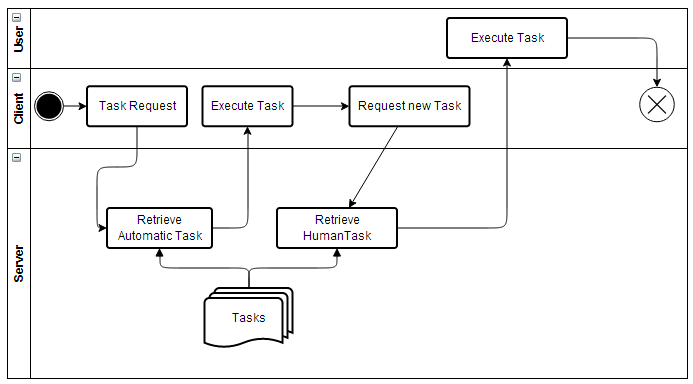
\includegraphics[width=\columnwidth]{Workflow}
    \caption{The conceptual Workflow handled by the framework.}
    \label{fig:workflow}
\end{figure}

In the \emph{Workflow Design} we must describe, at a conceptual level, how our
framework deals with the client and how the tasks are executed. During the
\emph{Data Design} we stated that the tasks can have relationships and thus our
framework must be able to handle different Task types seamlessly. In
\autoref{fig:workflow} is depicted a typical flow of execution of a Work (a
composition of Tasks) with multiple task types.\\

Our Workflow model must be able to handle the interleaving of human and automatic
task without any human intervention. The Workflow must take into account also the
constraints defined during the creation step and manage the execution of the
tasks accordingly.

A feature that the framework is required to handle is also the case where
the application type is not strictly human or strictly automatic. We can have
scenarios where the task is a blend of both human and automatic interactions.
\ac{GWAP} are a case where the automatic computation and the human interaction
are blended together. Other scenarios can be the validation of the automatically
computed results as we presented in our use case (see \ref{sec:cases:hybrid}).

To guarantee the needed flexibility the framework must be able to include third-part
logic in charge of managing certain steps of the execution (like Task planning).




\subsection{Framework Design}
In the design process of the framework we took all the conceptually designed data
and workflows, as well as the requirements, and we merged them together in order
to create the whole structure for supporting our framework.\\

During the \textbf{Data Design} we pointed out the data structures that
need to be managed. The \emph{Workflow Model} needs to specify the relationships
between the modules an the "connection points" where the third part softwares
are plugged. On top of that, every Task must have defined its set of input and
output data.
The \emph{Task Data Model} specifies all the data structure of the task, building
the metamodel for each Task. The metamodel contains all the information on the 
structure of the data model for a Task.
In the \emph{Task Model} there are contained all the actual data for each Task, called
Objects. Each object represents a "row" of the data and is, in turn,
associated to a Task.
The \emph{Task Execution Model} contains all the information on the actual
execution of a Task. It stores all the information on the user that performed the task and
the device used.\\

The \textbf{Workflow Design} allows us to create the software able to handle all
the different types of archetype application (e.g. Human computation, Automatic
computation) giving also the guidelines on how to manage the interaction between
subsequent Task execution.